\documentclass[1p]{elsarticle_modified}
%\bibliographystyle{elsarticle-num}

%\usepackage[colorlinks]{hyperref}
%\usepackage{abbrmath_seonhwa} %\Abb, \Ascr, \Acal ,\Abf, \Afrak
\usepackage{amsfonts}
\usepackage{amssymb}
\usepackage{amsmath}
\usepackage{amsthm}
\usepackage{scalefnt}
\usepackage{amsbsy}
\usepackage{kotex}
\usepackage{caption}
\usepackage{subfig}
\usepackage{color}
\usepackage{graphicx}
\usepackage{xcolor} %% white, black, red, green, blue, cyan, magenta, yellow
\usepackage{float}
\usepackage{setspace}
\usepackage{hyperref}

\usepackage{tikz}
\usetikzlibrary{arrows}

\usepackage{multirow}
\usepackage{array} % fixed length table
\usepackage{hhline}

%%%%%%%%%%%%%%%%%%%%%
\makeatletter
\renewcommand*\env@matrix[1][\arraystretch]{%
	\edef\arraystretch{#1}%
	\hskip -\arraycolsep
	\let\@ifnextchar\new@ifnextchar
	\array{*\c@MaxMatrixCols c}}
\makeatother %https://tex.stackexchange.com/questions/14071/how-can-i-increase-the-line-spacing-in-a-matrix
%%%%%%%%%%%%%%%

\usepackage[normalem]{ulem}

\newcommand{\msout}[1]{\ifmmode\text{\sout{\ensuremath{#1}}}\else\sout{#1}\fi}
%SOURCE: \msout is \stkout macro in https://tex.stackexchange.com/questions/20609/strikeout-in-math-mode

\newcommand{\cancel}[1]{
	\ifmmode
	{\color{red}\msout{#1}}
	\else
	{\color{red}\sout{#1}}
	\fi
}

\newcommand{\add}[1]{
	{\color{blue}\uwave{#1}}
}

\newcommand{\replace}[2]{
	\ifmmode
	{\color{red}\msout{#1}}{\color{blue}\uwave{#2}}
	\else
	{\color{red}\sout{#1}}{\color{blue}\uwave{#2}}
	\fi
}

\newcommand{\Sol}{\mathcal{S}} %segment
\newcommand{\D}{D} %diagram
\newcommand{\A}{\mathcal{A}} %arc


%%%%%%%%%%%%%%%%%%%%%%%%%%%%%5 test

\def\sl{\operatorname{\textup{SL}}(2,\Cbb)}
\def\psl{\operatorname{\textup{PSL}}(2,\Cbb)}
\def\quan{\mkern 1mu \triangleright \mkern 1mu}

\theoremstyle{definition}
\newtheorem{thm}{Theorem}[section]
\newtheorem{prop}[thm]{Proposition}
\newtheorem{lem}[thm]{Lemma}
\newtheorem{ques}[thm]{Question}
\newtheorem{cor}[thm]{Corollary}
\newtheorem{defn}[thm]{Definition}
\newtheorem{exam}[thm]{Example}
\newtheorem{rmk}[thm]{Remark}
\newtheorem{alg}[thm]{Algorithm}

\newcommand{\I}{\sqrt{-1}}
\begin{document}

%\begin{frontmatter}
%
%\title{Boundary parabolic representations of knots up to 8 crossings}
%
%%% Group authors per affiliation:
%\author{Yunhi Cho} 
%\address{Department of Mathematics, University of Seoul, Seoul, Korea}
%\ead{yhcho@uos.ac.kr}
%
%
%\author{Seonhwa Kim} %\fnref{s_kim}}
%\address{Center for Geometry and Physics, Institute for Basic Science, Pohang, 37673, Korea}
%\ead{ryeona17@ibs.re.kr}
%
%\author{Hyuk Kim}
%\address{Department of Mathematical Sciences, Seoul National University, Seoul 08826, Korea}
%\ead{hyukkim@snu.ac.kr}
%
%\author{Seokbeom Yoon}
%\address{Department of Mathematical Sciences, Seoul National University, Seoul, 08826,  Korea}
%\ead{sbyoon15@snu.ac.kr}
%
%\begin{abstract}
%We find all boundary parabolic representation of knots up to 8 crossings.
%
%\end{abstract}
%\begin{keyword}
%    \MSC[2010] 57M25 
%\end{keyword}
%
%\end{frontmatter}

%\linenumbers
%\tableofcontents
%
\newcommand\colored[1]{\textcolor{white}{\rule[-0.35ex]{0.8em}{1.4ex}}\kern-0.8em\color{red} #1}%
%\newcommand\colored[1]{\textcolor{white}{ #1}\kern-2.17ex	\textcolor{white}{ #1}\kern-1.81ex	\textcolor{white}{ #1}\kern-2.15ex\color{red}#1	}

{\Large $\underline{12n_{0618}~(K12n_{0618})}$}

\setlength{\tabcolsep}{10pt}
\renewcommand{\arraystretch}{1.6}
\vspace{1cm}\begin{tabular}{m{100pt}>{\centering\arraybackslash}m{274pt}}
\multirow{5}{120pt}{
	\centering
	\includegraphics[width=112pt]{../../../GIT/diagram.site/Diagrams/png/2707_12n_0618.png}\\
\ \ \ A knot diagram\footnotemark}&
\allowdisplaybreaks
\textbf{Linearized knot diagam} \\
\cline{2-2}
 &
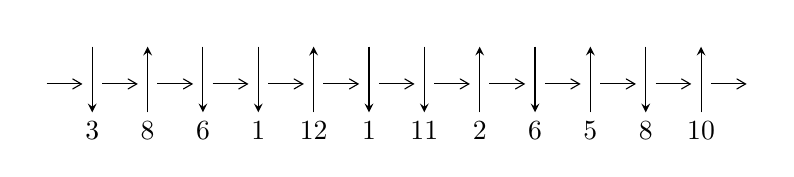
\begin{tikzpicture}[x=20pt, y=17pt]
	% nodes
	\node (C0) at (0, 0) {};
	\node (C1) at (1, 0) {};
	\node (C1U) at (1, +1) {};
	\node (C1D) at (1, -1) {3};

	\node (C2) at (2, 0) {};
	\node (C2U) at (2, +1) {};
	\node (C2D) at (2, -1) {8};

	\node (C3) at (3, 0) {};
	\node (C3U) at (3, +1) {};
	\node (C3D) at (3, -1) {6};

	\node (C4) at (4, 0) {};
	\node (C4U) at (4, +1) {};
	\node (C4D) at (4, -1) {1};

	\node (C5) at (5, 0) {};
	\node (C5U) at (5, +1) {};
	\node (C5D) at (5, -1) {12};

	\node (C6) at (6, 0) {};
	\node (C6U) at (6, +1) {};
	\node (C6D) at (6, -1) {1};

	\node (C7) at (7, 0) {};
	\node (C7U) at (7, +1) {};
	\node (C7D) at (7, -1) {11};

	\node (C8) at (8, 0) {};
	\node (C8U) at (8, +1) {};
	\node (C8D) at (8, -1) {2};

	\node (C9) at (9, 0) {};
	\node (C9U) at (9, +1) {};
	\node (C9D) at (9, -1) {6};

	\node (C10) at (10, 0) {};
	\node (C10U) at (10, +1) {};
	\node (C10D) at (10, -1) {5};

	\node (C11) at (11, 0) {};
	\node (C11U) at (11, +1) {};
	\node (C11D) at (11, -1) {8};

	\node (C12) at (12, 0) {};
	\node (C12U) at (12, +1) {};
	\node (C12D) at (12, -1) {10};
	\node (C13) at (13, 0) {};

	% arrows
	\draw[->,>={angle 60}]
	(C0) edge (C1) (C1) edge (C2) (C2) edge (C3) (C3) edge (C4) (C4) edge (C5) (C5) edge (C6) (C6) edge (C7) (C7) edge (C8) (C8) edge (C9) (C9) edge (C10) (C10) edge (C11) (C11) edge (C12) (C12) edge (C13) ;	\draw[->,>=stealth]
	(C1U) edge (C1D) (C2D) edge (C2U) (C3U) edge (C3D) (C4U) edge (C4D) (C5D) edge (C5U) (C6U) edge (C6D) (C7U) edge (C7D) (C8D) edge (C8U) (C9U) edge (C9D) (C10D) edge (C10U) (C11U) edge (C11D) (C12D) edge (C12U) ;
	\end{tikzpicture} \\
\hhline{~~} \\& 
\textbf{Solving Sequence} \\ \cline{2-2} 
 &
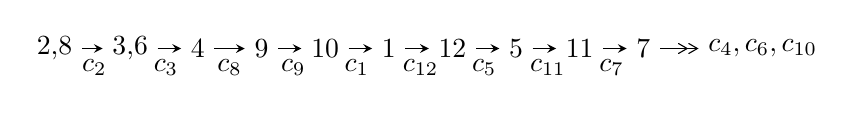
\begin{tikzpicture}[x=23pt, y=7pt]
	% node
	\node (A0) at (-1/8, 0) {2,8};
	\node (A1) at (17/16, 0) {3,6};
	\node (A2) at (17/8, 0) {4};
	\node (A3) at (25/8, 0) {9};
	\node (A4) at (33/8, 0) {10};
	\node (A5) at (41/8, 0) {1};
	\node (A6) at (49/8, 0) {12};
	\node (A7) at (57/8, 0) {5};
	\node (A8) at (65/8, 0) {11};
	\node (A9) at (73/8, 0) {7};
	\node (C1) at (1/2, -1) {$c_{2}$};
	\node (C2) at (13/8, -1) {$c_{3}$};
	\node (C3) at (21/8, -1) {$c_{8}$};
	\node (C4) at (29/8, -1) {$c_{9}$};
	\node (C5) at (37/8, -1) {$c_{1}$};
	\node (C6) at (45/8, -1) {$c_{12}$};
	\node (C7) at (53/8, -1) {$c_{5}$};
	\node (C8) at (61/8, -1) {$c_{11}$};
	\node (C9) at (69/8, -1) {$c_{7}$};
	\node (A10) at (11, 0) {$c_{4},c_{6},c_{10}$};

	% edge
	\draw[->,>=stealth]	
	(A0) edge (A1) (A1) edge (A2) (A2) edge (A3) (A3) edge (A4) (A4) edge (A5) (A5) edge (A6) (A6) edge (A7) (A7) edge (A8) (A8) edge (A9) ;
	\draw[->>,>={angle 60}]	
	(A9) edge (A10);
\end{tikzpicture} \\ 

\end{tabular} \\

\footnotetext{
The image of knot diagram is generated by the software ``\textbf{Draw programme}" developed by Andrew Bartholomew(\url{http://www.layer8.co.uk/maths/draw/index.htm\#Running-draw}), where we modified some parts for our purpose(\url{https://github.com/CATsTAILs/LinksPainter}).
}\phantom \\ \newline 
\centering \textbf{Ideals for irreducible components\footnotemark of $X_{\text{par}}$} 
 
\begin{align*}
I^u_{1}&=\langle 
2.78413\times10^{157} u^{83}+4.41545\times10^{158} u^{82}+\cdots+6.49095\times10^{157} b+2.25203\times10^{160},\\
\phantom{I^u_{1}}&\phantom{= \langle  }1.03935\times10^{160} u^{83}+1.05276\times10^{160} u^{82}+\cdots+3.18057\times10^{159} a+1.00444\times10^{162},\\
\phantom{I^u_{1}}&\phantom{= \langle  }u^{84}- u^{83}+\cdots-111 u+49\rangle \\
I^u_{2}&=\langle 
-5 u^{30}-2 u^{29}+\cdots+b-4,\;-3 u^{30}+2 u^{29}+\cdots+a-1,\;u^{31}+8 u^{29}+\cdots-4 u+1\rangle \\
\\
\end{align*}
\raggedright * 2 irreducible components of $\dim_{\mathbb{C}}=0$, with total 115 representations.\\
\footnotetext{All coefficients of polynomials are rational numbers. But the coefficients are sometimes approximated in decimal forms when there is not enough margin.}
\newpage
\renewcommand{\arraystretch}{1}
\centering \section*{I. $I^u_{1}= \langle 2.78\times10^{157} u^{83}+4.42\times10^{158} u^{82}+\cdots+6.49\times10^{157} b+2.25\times10^{160},\;1.04\times10^{160} u^{83}+1.05\times10^{160} u^{82}+\cdots+3.18\times10^{159} a+1.00\times10^{162},\;u^{84}- u^{83}+\cdots-111 u+49 \rangle$}
\flushleft \textbf{(i) Arc colorings}\\
\begin{tabular}{m{7pt} m{180pt} m{7pt} m{180pt} }
\flushright $a_{2}=$&$\begin{pmatrix}1\\0\end{pmatrix}$ \\
\flushright $a_{8}=$&$\begin{pmatrix}0\\u\end{pmatrix}$ \\
\flushright $a_{3}=$&$\begin{pmatrix}1\\- u^2\end{pmatrix}$ \\
\flushright $a_{6}=$&$\begin{pmatrix}-3.26781 u^{83}-3.30996 u^{82}+\cdots+487.028 u-315.806\\-0.428925 u^{83}-6.80246 u^{82}+\cdots+728.359 u-346.949\end{pmatrix}$ \\
\flushright $a_{4}=$&$\begin{pmatrix}-1.16716 u^{83}-1.19878 u^{82}+\cdots+112.821 u-87.6721\\0.148106 u^{83}-0.591608 u^{82}+\cdots+30.7174 u-25.5279\end{pmatrix}$ \\
\flushright $a_{9}=$&$\begin{pmatrix}u\\u\end{pmatrix}$ \\
\flushright $a_{10}=$&$\begin{pmatrix}-2.43860 u^{83}+2.86253 u^{82}+\cdots-210.519 u+45.7678\\-0.688297 u^{83}-0.498914 u^{82}+\cdots+43.5911 u-43.6754\end{pmatrix}$ \\
\flushright $a_{1}=$&$\begin{pmatrix}u^2+1\\- u^4\end{pmatrix}$ \\
\flushright $a_{12}=$&$\begin{pmatrix}5.77871 u^{83}-5.15966 u^{82}+\cdots+404.557 u-35.3569\\4.36764 u^{83}+3.76892 u^{82}+\cdots-546.433 u+386.589\end{pmatrix}$ \\
\flushright $a_{5}=$&$\begin{pmatrix}-0.405428 u^{83}-1.49265 u^{82}+\cdots+134.373 u-79.1284\\1.55554 u^{83}-2.95746 u^{82}+\cdots+251.078 u-103.417\end{pmatrix}$ \\
\flushright $a_{11}=$&$\begin{pmatrix}5.77871 u^{83}-5.15966 u^{82}+\cdots+404.557 u-35.3569\\9.19323 u^{83}+0.355636 u^{82}+\cdots-331.991 u+416.922\end{pmatrix}$ \\
\flushright $a_{7}=$&$\begin{pmatrix}-2.31774 u^{83}-3.78616 u^{82}+\cdots+504.281 u-305.207\\-0.356820 u^{83}-11.5652 u^{82}+\cdots+1284.14 u-608.102\end{pmatrix}$\\&\end{tabular}
\flushleft \textbf{(ii) Obstruction class $= -1$}\\~\\
\flushleft \textbf{(iii) Cusp Shapes $= -5.61656 u^{83}-5.45770 u^{82}+\cdots+670.848 u-462.720$}\\~\\
\newpage\renewcommand{\arraystretch}{1}
\flushleft \textbf{(iv) u-Polynomials at the component}\newline \\
\begin{tabular}{m{50pt}|m{274pt}}
Crossings & \hspace{64pt}u-Polynomials at each crossing \\
\hline $$\begin{aligned}c_{1}\end{aligned}$$&$\begin{aligned}
&u^{84}+51 u^{83}+\cdots+45793 u+2401
\end{aligned}$\\
\hline $$\begin{aligned}c_{2},c_{8}\end{aligned}$$&$\begin{aligned}
&u^{84}+u^{83}+\cdots+111 u+49
\end{aligned}$\\
\hline $$\begin{aligned}c_{3}\end{aligned}$$&$\begin{aligned}
&u^{84}+8 u^{83}+\cdots-11118 u+1361
\end{aligned}$\\
\hline $$\begin{aligned}c_{4}\end{aligned}$$&$\begin{aligned}
&u^{84}-9 u^{83}+\cdots-217846165 u+89630771
\end{aligned}$\\
\hline $$\begin{aligned}c_{5}\end{aligned}$$&$\begin{aligned}
&u^{84}-3 u^{83}+\cdots-1457 u+173
\end{aligned}$\\
\hline $$\begin{aligned}c_{6}\end{aligned}$$&$\begin{aligned}
&u^{84}-41 u^{82}+\cdots+1075379 u+53761
\end{aligned}$\\
\hline $$\begin{aligned}c_{7},c_{11}\end{aligned}$$&$\begin{aligned}
&u^{84}+u^{83}+\cdots+14 u+1
\end{aligned}$\\
\hline $$\begin{aligned}c_{9}\end{aligned}$$&$\begin{aligned}
&u^{84}+3 u^{83}+\cdots+5494435 u+643211
\end{aligned}$\\
\hline $$\begin{aligned}c_{10}\end{aligned}$$&$\begin{aligned}
&u^{84}+u^{83}+\cdots+7748 u+16641
\end{aligned}$\\
\hline $$\begin{aligned}c_{12}\end{aligned}$$&$\begin{aligned}
&u^{84}+4 u^{83}+\cdots+8 u+1
\end{aligned}$\\
\hline
\end{tabular}\\~\\
\newpage\renewcommand{\arraystretch}{1}
\flushleft \textbf{(v) Riley Polynomials at the component}\newline \\
\begin{tabular}{m{50pt}|m{274pt}}
Crossings & \hspace{64pt}Riley Polynomials at each crossing \\
\hline $$\begin{aligned}c_{1}\end{aligned}$$&$\begin{aligned}
&y^{84}-25 y^{83}+\cdots+451388937 y+5764801
\end{aligned}$\\
\hline $$\begin{aligned}c_{2},c_{8}\end{aligned}$$&$\begin{aligned}
&y^{84}+51 y^{83}+\cdots+45793 y+2401
\end{aligned}$\\
\hline $$\begin{aligned}c_{3}\end{aligned}$$&$\begin{aligned}
&y^{84}-94 y^{83}+\cdots+3281550 y+1852321
\end{aligned}$\\
\hline $$\begin{aligned}c_{4}\end{aligned}$$&$\begin{aligned}
&y^{84}-69 y^{83}+\cdots-93715556363356613 y+8033675110054441
\end{aligned}$\\
\hline $$\begin{aligned}c_{5}\end{aligned}$$&$\begin{aligned}
&y^{84}+19 y^{83}+\cdots-9004789 y+29929
\end{aligned}$\\
\hline $$\begin{aligned}c_{6}\end{aligned}$$&$\begin{aligned}
&y^{84}-82 y^{83}+\cdots-150205571231 y+2890245121
\end{aligned}$\\
\hline $$\begin{aligned}c_{7},c_{11}\end{aligned}$$&$\begin{aligned}
&y^{84}-63 y^{83}+\cdots-68 y+1
\end{aligned}$\\
\hline $$\begin{aligned}c_{9}\end{aligned}$$&$\begin{aligned}
&y^{84}-47 y^{83}+\cdots+6919320761307 y+413720390521
\end{aligned}$\\
\hline $$\begin{aligned}c_{10}\end{aligned}$$&$\begin{aligned}
&y^{84}+23 y^{83}+\cdots+12729508892 y+276922881
\end{aligned}$\\
\hline $$\begin{aligned}c_{12}\end{aligned}$$&$\begin{aligned}
&y^{84}+6 y^{83}+\cdots+104 y+1
\end{aligned}$\\
\hline
\end{tabular}\\~\\
\newpage\flushleft \textbf{(vi) Complex Volumes and Cusp Shapes}
$$\begin{array}{c|c|c}  
\text{Solutions to }I^u_{1}& \I (\text{vol} + \sqrt{-1}CS) & \text{Cusp shape}\\
 \hline 
\begin{aligned}
u &= \phantom{-}0.624339 + 0.776376 I \\
a &= -0.402447 + 0.827895 I \\
b &= \phantom{-}0.577955 + 0.944921 I\end{aligned}
 & \phantom{-}2.98746 - 1.05041 I & \phantom{-0.000000 } 0 \\ \hline\begin{aligned}
u &= \phantom{-}0.624339 - 0.776376 I \\
a &= -0.402447 - 0.827895 I \\
b &= \phantom{-}0.577955 - 0.944921 I\end{aligned}
 & \phantom{-}2.98746 + 1.05041 I & \phantom{-0.000000 } 0 \\ \hline\begin{aligned}
u &= -0.984757 + 0.028992 I \\
a &= -1.305870 - 0.531353 I \\
b &= -0.167274 + 0.135617 I\end{aligned}
 & -3.43240 - 4.70886 I & \phantom{-0.000000 } 0 \\ \hline\begin{aligned}
u &= -0.984757 - 0.028992 I \\
a &= -1.305870 + 0.531353 I \\
b &= -0.167274 - 0.135617 I\end{aligned}
 & -3.43240 + 4.70886 I & \phantom{-0.000000 } 0 \\ \hline\begin{aligned}
u &= \phantom{-}0.070205 + 0.974127 I \\
a &= \phantom{-}0.676828 - 0.681396 I \\
b &= -0.77441 - 1.73440 I\end{aligned}
 & -0.62510 + 3.04588 I & \phantom{-0.000000 } 0 \\ \hline\begin{aligned}
u &= \phantom{-}0.070205 - 0.974127 I \\
a &= \phantom{-}0.676828 + 0.681396 I \\
b &= -0.77441 + 1.73440 I\end{aligned}
 & -0.62510 - 3.04588 I & \phantom{-0.000000 } 0 \\ \hline\begin{aligned}
u &= \phantom{-}0.152041 + 1.034940 I \\
a &= -1.074540 - 0.801428 I \\
b &= \phantom{-}0.312399 - 0.793279 I\end{aligned}
 & -5.11490 + 2.83585 I & \phantom{-0.000000 } 0 \\ \hline\begin{aligned}
u &= \phantom{-}0.152041 - 1.034940 I \\
a &= -1.074540 + 0.801428 I \\
b &= \phantom{-}0.312399 + 0.793279 I\end{aligned}
 & -5.11490 - 2.83585 I & \phantom{-0.000000 } 0 \\ \hline\begin{aligned}
u &= \phantom{-}0.057583 + 0.947885 I \\
a &= -0.93954 + 2.00808 I \\
b &= -0.21235 + 2.27623 I\end{aligned}
 & \phantom{-}1.035170 + 0.344979 I & \phantom{-0.000000 } 0 \\ \hline\begin{aligned}
u &= \phantom{-}0.057583 - 0.947885 I \\
a &= -0.93954 - 2.00808 I \\
b &= -0.21235 - 2.27623 I\end{aligned}
 & \phantom{-}1.035170 - 0.344979 I & \phantom{-0.000000 } 0\\
 \hline 
 \end{array}$$\newpage$$\begin{array}{c|c|c}  
\text{Solutions to }I^u_{1}& \I (\text{vol} + \sqrt{-1}CS) & \text{Cusp shape}\\
 \hline 
\begin{aligned}
u &= \phantom{-}1.056600 + 0.170943 I \\
a &= -1.159070 + 0.193628 I \\
b &= -0.127728 + 0.182476 I\end{aligned}
 & -7.93661 - 2.97178 I & \phantom{-0.000000 } 0 \\ \hline\begin{aligned}
u &= \phantom{-}1.056600 - 0.170943 I \\
a &= -1.159070 - 0.193628 I \\
b &= -0.127728 - 0.182476 I\end{aligned}
 & -7.93661 + 2.97178 I & \phantom{-0.000000 } 0 \\ \hline\begin{aligned}
u &= \phantom{-}1.064760 + 0.140239 I \\
a &= -1.61256 - 0.31819 I \\
b &= -0.007697 + 0.448028 I\end{aligned}
 & -8.8561 - 11.2574 I & \phantom{-0.000000 } 0 \\ \hline\begin{aligned}
u &= \phantom{-}1.064760 - 0.140239 I \\
a &= -1.61256 + 0.31819 I \\
b &= -0.007697 - 0.448028 I\end{aligned}
 & -8.8561 + 11.2574 I & \phantom{-0.000000 } 0 \\ \hline\begin{aligned}
u &= \phantom{-}0.266496 + 0.883595 I \\
a &= -1.17684 - 2.39946 I \\
b &= -1.07953 - 2.21939 I\end{aligned}
 & -2.41310 + 6.12076 I & \phantom{-0.000000 } 0. - 7.70810 I \\ \hline\begin{aligned}
u &= \phantom{-}0.266496 - 0.883595 I \\
a &= -1.17684 + 2.39946 I \\
b &= -1.07953 + 2.21939 I\end{aligned}
 & -2.41310 - 6.12076 I & \phantom{-0.000000 -}0. + 7.70810 I \\ \hline\begin{aligned}
u &= -0.618147 + 0.892022 I \\
a &= \phantom{-}0.240538 - 0.019613 I \\
b &= -0.764502 - 0.092969 I\end{aligned}
 & -2.45152 + 0.05749 I & \phantom{-0.000000 } 0 \\ \hline\begin{aligned}
u &= -0.618147 - 0.892022 I \\
a &= \phantom{-}0.240538 + 0.019613 I \\
b &= -0.764502 + 0.092969 I\end{aligned}
 & -2.45152 - 0.05749 I & \phantom{-0.000000 } 0 \\ \hline\begin{aligned}
u &= \phantom{-}0.400936 + 1.008700 I \\
a &= \phantom{-}0.099014 - 1.279680 I \\
b &= -0.25180 - 2.23090 I\end{aligned}
 & -3.64938 + 5.14792 I & \phantom{-0.000000 } 0 \\ \hline\begin{aligned}
u &= \phantom{-}0.400936 - 1.008700 I \\
a &= \phantom{-}0.099014 + 1.279680 I \\
b &= -0.25180 + 2.23090 I\end{aligned}
 & -3.64938 - 5.14792 I & \phantom{-0.000000 } 0\\
 \hline 
 \end{array}$$\newpage$$\begin{array}{c|c|c}  
\text{Solutions to }I^u_{1}& \I (\text{vol} + \sqrt{-1}CS) & \text{Cusp shape}\\
 \hline 
\begin{aligned}
u &= -0.252494 + 0.875622 I \\
a &= \phantom{-}0.960910 - 0.430174 I \\
b &= \phantom{-}0.601016 - 0.096506 I\end{aligned}
 & -0.43979 - 1.58507 I & \phantom{-0.000000 -}0. + 4.81532 I \\ \hline\begin{aligned}
u &= -0.252494 - 0.875622 I \\
a &= \phantom{-}0.960910 + 0.430174 I \\
b &= \phantom{-}0.601016 + 0.096506 I\end{aligned}
 & -0.43979 + 1.58507 I & \phantom{-0.000000 } 0. - 4.81532 I \\ \hline\begin{aligned}
u &= -0.855464 + 0.674714 I \\
a &= \phantom{-}0.028517 - 0.741459 I \\
b &= \phantom{-}0.571683 + 0.220653 I\end{aligned}
 & -0.681532 + 0.899140 I & \phantom{-0.000000 } 0 \\ \hline\begin{aligned}
u &= -0.855464 - 0.674714 I \\
a &= \phantom{-}0.028517 + 0.741459 I \\
b &= \phantom{-}0.571683 - 0.220653 I\end{aligned}
 & -0.681532 - 0.899140 I & \phantom{-0.000000 } 0 \\ \hline\begin{aligned}
u &= -0.155261 + 1.079100 I \\
a &= -0.325368 + 0.475644 I \\
b &= -0.34063 + 1.77064 I\end{aligned}
 & -2.09724 - 2.85559 I & \phantom{-0.000000 } 0 \\ \hline\begin{aligned}
u &= -0.155261 - 1.079100 I \\
a &= -0.325368 - 0.475644 I \\
b &= -0.34063 - 1.77064 I\end{aligned}
 & -2.09724 + 2.85559 I & \phantom{-0.000000 } 0 \\ \hline\begin{aligned}
u &= \phantom{-}0.621232 + 0.914123 I \\
a &= -0.876179 + 0.130572 I \\
b &= -0.478088 + 0.940852 I\end{aligned}
 & \phantom{-}2.55309 + 5.96851 I & \phantom{-0.000000 } 0 \\ \hline\begin{aligned}
u &= \phantom{-}0.621232 - 0.914123 I \\
a &= -0.876179 - 0.130572 I \\
b &= -0.478088 - 0.940852 I\end{aligned}
 & \phantom{-}2.55309 - 5.96851 I & \phantom{-0.000000 } 0 \\ \hline\begin{aligned}
u &= -0.889487 + 0.087296 I \\
a &= \phantom{-}1.49853 + 0.36339 I \\
b &= \phantom{-}0.478615 + 0.423569 I\end{aligned}
 & -7.16342 - 1.69036 I & -8.17295 + 4.28512 I \\ \hline\begin{aligned}
u &= -0.889487 - 0.087296 I \\
a &= \phantom{-}1.49853 - 0.36339 I \\
b &= \phantom{-}0.478615 - 0.423569 I\end{aligned}
 & -7.16342 + 1.69036 I & -8.17295 - 4.28512 I\\
 \hline 
 \end{array}$$\newpage$$\begin{array}{c|c|c}  
\text{Solutions to }I^u_{1}& \I (\text{vol} + \sqrt{-1}CS) & \text{Cusp shape}\\
 \hline 
\begin{aligned}
u &= \phantom{-}0.099728 + 0.867946 I \\
a &= \phantom{-}0.624002 - 0.596405 I \\
b &= -0.691779 - 0.310908 I\end{aligned}
 & -0.40378 - 2.13241 I & -4.45473 + 4.83431 I \\ \hline\begin{aligned}
u &= \phantom{-}0.099728 - 0.867946 I \\
a &= \phantom{-}0.624002 + 0.596405 I \\
b &= -0.691779 + 0.310908 I\end{aligned}
 & -0.40378 + 2.13241 I & -4.45473 - 4.83431 I \\ \hline\begin{aligned}
u &= -0.344209 + 0.802582 I \\
a &= \phantom{-}0.954239 + 0.172222 I \\
b &= \phantom{-}0.469133 + 0.722529 I\end{aligned}
 & -0.30736 - 1.52896 I & -2.00000 + 5.06207 I \\ \hline\begin{aligned}
u &= -0.344209 - 0.802582 I \\
a &= \phantom{-}0.954239 - 0.172222 I \\
b &= \phantom{-}0.469133 - 0.722529 I\end{aligned}
 & -0.30736 + 1.52896 I & -2.00000 - 5.06207 I \\ \hline\begin{aligned}
u &= \phantom{-}0.521057 + 0.696756 I \\
a &= \phantom{-}2.25645 + 0.55350 I \\
b &= \phantom{-}1.84405 - 0.56915 I\end{aligned}
 & -2.02874 - 2.80140 I & -3.16614 + 3.38466 I \\ \hline\begin{aligned}
u &= \phantom{-}0.521057 - 0.696756 I \\
a &= \phantom{-}2.25645 - 0.55350 I \\
b &= \phantom{-}1.84405 + 0.56915 I\end{aligned}
 & -2.02874 + 2.80140 I & -3.16614 - 3.38466 I \\ \hline\begin{aligned}
u &= -1.129490 + 0.150367 I \\
a &= \phantom{-}1.80812 - 0.45022 I \\
b &= -0.505344 + 0.948878 I\end{aligned}
 & -6.41608 + 0.87005 I & \phantom{-0.000000 } 0 \\ \hline\begin{aligned}
u &= -1.129490 - 0.150367 I \\
a &= \phantom{-}1.80812 + 0.45022 I \\
b &= -0.505344 - 0.948878 I\end{aligned}
 & -6.41608 - 0.87005 I & \phantom{-0.000000 } 0 \\ \hline\begin{aligned}
u &= \phantom{-}0.317066 + 1.096700 I \\
a &= -0.80464 - 1.22601 I \\
b &= -0.73642 - 2.85554 I\end{aligned}
 & -4.04887 + 7.70346 I & \phantom{-0.000000 } 0 \\ \hline\begin{aligned}
u &= \phantom{-}0.317066 - 1.096700 I \\
a &= -0.80464 + 1.22601 I \\
b &= -0.73642 + 2.85554 I\end{aligned}
 & -4.04887 - 7.70346 I & \phantom{-0.000000 } 0\\
 \hline 
 \end{array}$$\newpage$$\begin{array}{c|c|c}  
\text{Solutions to }I^u_{1}& \I (\text{vol} + \sqrt{-1}CS) & \text{Cusp shape}\\
 \hline 
\begin{aligned}
u &= -0.231757 + 1.181000 I \\
a &= -0.730973 - 1.200560 I \\
b &= \phantom{-}0.07606 - 1.88946 I\end{aligned}
 & -5.80217 - 6.52422 I & \phantom{-0.000000 } 0 \\ \hline\begin{aligned}
u &= -0.231757 - 1.181000 I \\
a &= -0.730973 + 1.200560 I \\
b &= \phantom{-}0.07606 + 1.88946 I\end{aligned}
 & -5.80217 + 6.52422 I & \phantom{-0.000000 } 0 \\ \hline\begin{aligned}
u &= \phantom{-}0.793678 + 0.911216 I \\
a &= -0.083385 + 0.248184 I \\
b &= -0.386082 + 0.069923 I\end{aligned}
 & \phantom{-}5.63036 + 2.99540 I & \phantom{-0.000000 } 0 \\ \hline\begin{aligned}
u &= \phantom{-}0.793678 - 0.911216 I \\
a &= -0.083385 - 0.248184 I \\
b &= -0.386082 - 0.069923 I\end{aligned}
 & \phantom{-}5.63036 - 2.99540 I & \phantom{-0.000000 } 0 \\ \hline\begin{aligned}
u &= \phantom{-}0.279077 + 0.740387 I \\
a &= \phantom{-}1.271060 - 0.044685 I \\
b &= \phantom{-}1.87377 + 0.06065 I\end{aligned}
 & -4.18434 - 0.93777 I & -10.44340 - 1.29773 I \\ \hline\begin{aligned}
u &= \phantom{-}0.279077 - 0.740387 I \\
a &= \phantom{-}1.271060 + 0.044685 I \\
b &= \phantom{-}1.87377 - 0.06065 I\end{aligned}
 & -4.18434 + 0.93777 I & -10.44340 + 1.29773 I \\ \hline\begin{aligned}
u &= \phantom{-}0.769600 + 0.104576 I \\
a &= \phantom{-}1.88696 + 0.52531 I \\
b &= \phantom{-}0.429347 - 0.248742 I\end{aligned}
 & -2.63396 - 1.15147 I & -2.64253 - 2.45768 I \\ \hline\begin{aligned}
u &= \phantom{-}0.769600 - 0.104576 I \\
a &= \phantom{-}1.88696 - 0.52531 I \\
b &= \phantom{-}0.429347 + 0.248742 I\end{aligned}
 & -2.63396 + 1.15147 I & -2.64253 + 2.45768 I \\ \hline\begin{aligned}
u &= \phantom{-}0.416078 + 1.182460 I \\
a &= \phantom{-}0.208724 - 1.368180 I \\
b &= \phantom{-}0.86755 - 2.06309 I\end{aligned}
 & -6.34523 + 2.87444 I & \phantom{-0.000000 } 0 \\ \hline\begin{aligned}
u &= \phantom{-}0.416078 - 1.182460 I \\
a &= \phantom{-}0.208724 + 1.368180 I \\
b &= \phantom{-}0.86755 + 2.06309 I\end{aligned}
 & -6.34523 - 2.87444 I & \phantom{-0.000000 } 0\\
 \hline 
 \end{array}$$\newpage$$\begin{array}{c|c|c}  
\text{Solutions to }I^u_{1}& \I (\text{vol} + \sqrt{-1}CS) & \text{Cusp shape}\\
 \hline 
\begin{aligned}
u &= -0.498312 + 0.543146 I \\
a &= \phantom{-}0.125771 - 0.693418 I \\
b &= -0.062607 + 1.020890 I\end{aligned}
 & -1.56776 - 4.58591 I & -3.52776 + 6.17506 I \\ \hline\begin{aligned}
u &= -0.498312 - 0.543146 I \\
a &= \phantom{-}0.125771 + 0.693418 I \\
b &= -0.062607 - 1.020890 I\end{aligned}
 & -1.56776 + 4.58591 I & -3.52776 - 6.17506 I \\ \hline\begin{aligned}
u &= -0.116360 + 1.267120 I \\
a &= \phantom{-}0.225728 - 0.913470 I \\
b &= \phantom{-}1.07436 - 2.04992 I\end{aligned}
 & -7.20975 - 0.95387 I & \phantom{-0.000000 } 0 \\ \hline\begin{aligned}
u &= -0.116360 - 1.267120 I \\
a &= \phantom{-}0.225728 + 0.913470 I \\
b &= \phantom{-}1.07436 + 2.04992 I\end{aligned}
 & -7.20975 + 0.95387 I & \phantom{-0.000000 } 0 \\ \hline\begin{aligned}
u &= -0.802349 + 1.014890 I \\
a &= -0.394246 + 0.208156 I \\
b &= -1.092340 - 0.494974 I\end{aligned}
 & -1.65167 - 7.02055 I & \phantom{-0.000000 } 0 \\ \hline\begin{aligned}
u &= -0.802349 - 1.014890 I \\
a &= -0.394246 - 0.208156 I \\
b &= -1.092340 + 0.494974 I\end{aligned}
 & -1.65167 + 7.02055 I & \phantom{-0.000000 } 0 \\ \hline\begin{aligned}
u &= \phantom{-}0.489018 + 1.198890 I \\
a &= -0.10819 - 1.72417 I \\
b &= -0.36299 - 2.86624 I\end{aligned}
 & -5.84133 + 5.81556 I & \phantom{-0.000000 } 0 \\ \hline\begin{aligned}
u &= \phantom{-}0.489018 - 1.198890 I \\
a &= -0.10819 + 1.72417 I \\
b &= -0.36299 + 2.86624 I\end{aligned}
 & -5.84133 - 5.81556 I & \phantom{-0.000000 } 0 \\ \hline\begin{aligned}
u &= -0.433364 + 1.274080 I \\
a &= -0.425292 + 1.337080 I \\
b &= -0.12528 + 2.11785 I\end{aligned}
 & -11.30970 - 6.31124 I & \phantom{-0.000000 } 0 \\ \hline\begin{aligned}
u &= -0.433364 - 1.274080 I \\
a &= -0.425292 - 1.337080 I \\
b &= -0.12528 - 2.11785 I\end{aligned}
 & -11.30970 + 6.31124 I & \phantom{-0.000000 } 0\\
 \hline 
 \end{array}$$\newpage$$\begin{array}{c|c|c}  
\text{Solutions to }I^u_{1}& \I (\text{vol} + \sqrt{-1}CS) & \text{Cusp shape}\\
 \hline 
\begin{aligned}
u &= -0.524149 + 1.250560 I \\
a &= \phantom{-}0.39005 + 1.42843 I \\
b &= \phantom{-}0.39342 + 2.16528 I\end{aligned}
 & -10.64430 - 3.42952 I & \phantom{-0.000000 } 0 \\ \hline\begin{aligned}
u &= -0.524149 - 1.250560 I \\
a &= \phantom{-}0.39005 - 1.42843 I \\
b &= \phantom{-}0.39342 - 2.16528 I\end{aligned}
 & -10.64430 + 3.42952 I & \phantom{-0.000000 } 0 \\ \hline\begin{aligned}
u &= \phantom{-}0.519821 + 0.374551 I \\
a &= \phantom{-}1.88837 + 0.04418 I \\
b &= \phantom{-}0.179300 - 0.260934 I\end{aligned}
 & -1.87796 - 1.43458 I & -1.46731 - 0.52130 I \\ \hline\begin{aligned}
u &= \phantom{-}0.519821 - 0.374551 I \\
a &= \phantom{-}1.88837 - 0.04418 I \\
b &= \phantom{-}0.179300 + 0.260934 I\end{aligned}
 & -1.87796 + 1.43458 I & -1.46731 + 0.52130 I \\ \hline\begin{aligned}
u &= -0.486780 + 1.316210 I \\
a &= \phantom{-}0.140717 - 1.395610 I \\
b &= \phantom{-}0.40034 - 2.51194 I\end{aligned}
 & -7.59451 - 9.91142 I & \phantom{-0.000000 } 0 \\ \hline\begin{aligned}
u &= -0.486780 - 1.316210 I \\
a &= \phantom{-}0.140717 + 1.395610 I \\
b &= \phantom{-}0.40034 + 2.51194 I\end{aligned}
 & -7.59451 + 9.91142 I & \phantom{-0.000000 } 0 \\ \hline\begin{aligned}
u &= -0.51542 + 1.32110 I \\
a &= -0.251208 - 0.923395 I \\
b &= -0.74651 - 1.69422 I\end{aligned}
 & -7.40945 - 0.67992 I & \phantom{-0.000000 } 0 \\ \hline\begin{aligned}
u &= -0.51542 - 1.32110 I \\
a &= -0.251208 + 0.923395 I \\
b &= -0.74651 + 1.69422 I\end{aligned}
 & -7.40945 + 0.67992 I & \phantom{-0.000000 } 0 \\ \hline\begin{aligned}
u &= \phantom{-}0.58449 + 1.30757 I \\
a &= -0.14518 + 1.53271 I \\
b &= \phantom{-}0.23231 + 2.91128 I\end{aligned}
 & -12.4841 + 17.1391 I & \phantom{-0.000000 } 0 \\ \hline\begin{aligned}
u &= \phantom{-}0.58449 - 1.30757 I \\
a &= -0.14518 - 1.53271 I \\
b &= \phantom{-}0.23231 - 2.91128 I\end{aligned}
 & -12.4841 - 17.1391 I & \phantom{-0.000000 } 0\\
 \hline 
 \end{array}$$\newpage$$\begin{array}{c|c|c}  
\text{Solutions to }I^u_{1}& \I (\text{vol} + \sqrt{-1}CS) & \text{Cusp shape}\\
 \hline 
\begin{aligned}
u &= \phantom{-}0.59528 + 1.30604 I \\
a &= -0.194602 + 1.083090 I \\
b &= -0.22396 + 1.95074 I\end{aligned}
 & -11.4630 + 8.9032 I & \phantom{-0.000000 } 0 \\ \hline\begin{aligned}
u &= \phantom{-}0.59528 - 1.30604 I \\
a &= -0.194602 - 1.083090 I \\
b &= -0.22396 - 1.95074 I\end{aligned}
 & -11.4630 - 8.9032 I & \phantom{-0.000000 } 0 \\ \hline\begin{aligned}
u &= \phantom{-}0.38684 + 1.38887 I \\
a &= \phantom{-}0.162602 + 1.055620 I \\
b &= -0.00363 + 2.00199 I\end{aligned}
 & -13.05160 + 2.06430 I & \phantom{-0.000000 } 0 \\ \hline\begin{aligned}
u &= \phantom{-}0.38684 - 1.38887 I \\
a &= \phantom{-}0.162602 - 1.055620 I \\
b &= -0.00363 - 2.00199 I\end{aligned}
 & -13.05160 - 2.06430 I & \phantom{-0.000000 } 0 \\ \hline\begin{aligned}
u &= \phantom{-}0.40196 + 1.41075 I \\
a &= -0.265295 + 0.937006 I \\
b &= -1.15968 + 2.03447 I\end{aligned}
 & -13.9236 - 6.0378 I & \phantom{-0.000000 } 0 \\ \hline\begin{aligned}
u &= \phantom{-}0.40196 - 1.41075 I \\
a &= -0.265295 - 0.937006 I \\
b &= -1.15968 - 2.03447 I\end{aligned}
 & -13.9236 + 6.0378 I & \phantom{-0.000000 } 0 \\ \hline\begin{aligned}
u &= -0.39976 + 1.41147 I \\
a &= \phantom{-}0.524178 + 0.697717 I \\
b &= \phantom{-}2.23400 + 1.98841 I\end{aligned}
 & -11.64390 - 4.47794 I & \phantom{-0.000000 } 0 \\ \hline\begin{aligned}
u &= -0.39976 - 1.41147 I \\
a &= \phantom{-}0.524178 - 0.697717 I \\
b &= \phantom{-}2.23400 - 1.98841 I\end{aligned}
 & -11.64390 + 4.47794 I & \phantom{-0.000000 } 0 \\ \hline\begin{aligned}
u &= -0.59023 + 1.35145 I \\
a &= \phantom{-}0.29506 + 1.50766 I \\
b &= -0.38369 + 3.36097 I\end{aligned}
 & -10.23170 - 7.02272 I & \phantom{-0.000000 } 0 \\ \hline\begin{aligned}
u &= -0.59023 - 1.35145 I \\
a &= \phantom{-}0.29506 - 1.50766 I \\
b &= -0.38369 - 3.36097 I\end{aligned}
 & -10.23170 + 7.02272 I & \phantom{-0.000000 } 0\\
 \hline 
 \end{array}$$\newpage$$\begin{array}{c|c|c}  
\text{Solutions to }I^u_{1}& \I (\text{vol} + \sqrt{-1}CS) & \text{Cusp shape}\\
 \hline 
\begin{aligned}
u &= -0.383340 + 0.185448 I \\
a &= \phantom{-}0.37154 + 1.61335 I \\
b &= -0.338406 + 0.477813 I\end{aligned}
 & \phantom{-}1.21335 - 1.11387 I & \phantom{-}4.27095 + 2.48493 I \\ \hline\begin{aligned}
u &= -0.383340 - 0.185448 I \\
a &= \phantom{-}0.37154 - 1.61335 I \\
b &= -0.338406 - 0.477813 I\end{aligned}
 & \phantom{-}1.21335 + 1.11387 I & \phantom{-}4.27095 - 2.48493 I \\ \hline\begin{aligned}
u &= \phantom{-}0.223249 + 0.317821 I \\
a &= \phantom{-}3.38242 - 0.25747 I \\
b &= \phantom{-}0.407420 + 0.951931 I\end{aligned}
 & -1.76322 - 4.93035 I & -2.22330 + 7.33828 I \\ \hline\begin{aligned}
u &= \phantom{-}0.223249 - 0.317821 I \\
a &= \phantom{-}3.38242 + 0.25747 I \\
b &= \phantom{-}0.407420 - 0.951931 I\end{aligned}
 & -1.76322 + 4.93035 I & -2.22330 - 7.33828 I\\
 \hline 
 \end{array}$$\newpage\newpage\renewcommand{\arraystretch}{1}
\centering \section*{II. $I^u_{2}= \langle -5 u^{30}-2 u^{29}+\cdots+b-4,\;-3 u^{30}+2 u^{29}+\cdots+a-1,\;u^{31}+8 u^{29}+\cdots-4 u+1 \rangle$}
\flushleft \textbf{(i) Arc colorings}\\
\begin{tabular}{m{7pt} m{180pt} m{7pt} m{180pt} }
\flushright $a_{2}=$&$\begin{pmatrix}1\\0\end{pmatrix}$ \\
\flushright $a_{8}=$&$\begin{pmatrix}0\\u\end{pmatrix}$ \\
\flushright $a_{3}=$&$\begin{pmatrix}1\\- u^2\end{pmatrix}$ \\
\flushright $a_{6}=$&$\begin{pmatrix}3 u^{30}-2 u^{29}+\cdots+4 u+1\\5 u^{30}+2 u^{29}+\cdots-10 u+4\end{pmatrix}$ \\
\flushright $a_{4}=$&$\begin{pmatrix}2 u^{30}+3 u^{29}+\cdots-10 u+4\\6 u^{30}-6 u^{29}+\cdots+43 u-7\end{pmatrix}$ \\
\flushright $a_{9}=$&$\begin{pmatrix}u\\u\end{pmatrix}$ \\
\flushright $a_{10}=$&$\begin{pmatrix}4 u^{30}+u^{29}+\cdots-8 u+3\\-5 u^{30}+3 u^{29}+\cdots+7 u-3\end{pmatrix}$ \\
\flushright $a_{1}=$&$\begin{pmatrix}u^2+1\\- u^4\end{pmatrix}$ \\
\flushright $a_{12}=$&$\begin{pmatrix}2 u^{30}+6 u^{29}+\cdots-20 u+5\\-8 u^{30}+u^{29}+\cdots+16 u-6\end{pmatrix}$ \\
\flushright $a_{5}=$&$\begin{pmatrix}- u^{30}+u^{29}+\cdots+4 u-1\\6 u^{30}-9 u^{29}+\cdots+55 u-9\end{pmatrix}$ \\
\flushright $a_{11}=$&$\begin{pmatrix}2 u^{30}+6 u^{29}+\cdots-20 u+5\\-7 u^{30}+3 u^{29}+\cdots+27 u^2-6 u\end{pmatrix}$ \\
\flushright $a_{7}=$&$\begin{pmatrix}3 u^{30}-2 u^{29}+\cdots-27 u^2+4 u\\4 u^{30}+2 u^{29}+\cdots-11 u+4\end{pmatrix}$\\&\end{tabular}
\flushleft \textbf{(ii) Obstruction class $= 1$}\\~\\
\flushleft \textbf{(iii) Cusp Shapes $= -3 u^{29}-14 u^{28}-28 u^{27}-96 u^{26}-127 u^{25}-356 u^{24}-374 u^{23}-870 u^{22}-790 u^{21}-1557 u^{20}-1273 u^{19}-2066 u^{18}-1619 u^{17}-2021 u^{16}-1648 u^{15}-1324 u^{14}-1375 u^{13}-374 u^{12}-963 u^{11}+280 u^{10}-574 u^9+404 u^8-295 u^7+198 u^6-109 u^5+12 u^4-2 u^3-33 u^2+19 u-14$}\\~\\
\newpage\renewcommand{\arraystretch}{1}
\flushleft \textbf{(iv) u-Polynomials at the component}\newline \\
\begin{tabular}{m{50pt}|m{274pt}}
Crossings & \hspace{64pt}u-Polynomials at each crossing \\
\hline $$\begin{aligned}c_{1}\end{aligned}$$&$\begin{aligned}
&u^{31}-16 u^{30}+\cdots-8 u+1
\end{aligned}$\\
\hline $$\begin{aligned}c_{2}\end{aligned}$$&$\begin{aligned}
&u^{31}+8 u^{29}+\cdots-4 u+1
\end{aligned}$\\
\hline $$\begin{aligned}c_{3}\end{aligned}$$&$\begin{aligned}
&u^{31}-17 u^{30}+\cdots+543 u-71
\end{aligned}$\\
\hline $$\begin{aligned}c_{4}\end{aligned}$$&$\begin{aligned}
&u^{31}+4 u^{30}+\cdots+292 u+149
\end{aligned}$\\
\hline $$\begin{aligned}c_{5}\end{aligned}$$&$\begin{aligned}
&u^{31}-2 u^{29}+\cdots+2 u+1
\end{aligned}$\\
\hline $$\begin{aligned}c_{6}\end{aligned}$$&$\begin{aligned}
&u^{31}- u^{30}+\cdots+4 u+1
\end{aligned}$\\
\hline $$\begin{aligned}c_{7}\end{aligned}$$&$\begin{aligned}
&u^{31}-7 u^{29}+\cdots- u-1
\end{aligned}$\\
\hline $$\begin{aligned}c_{8}\end{aligned}$$&$\begin{aligned}
&u^{31}+8 u^{29}+\cdots-4 u-1
\end{aligned}$\\
\hline $$\begin{aligned}c_{9}\end{aligned}$$&$\begin{aligned}
&u^{31}-3 u^{29}+\cdots-2 u-1
\end{aligned}$\\
\hline $$\begin{aligned}c_{10}\end{aligned}$$&$\begin{aligned}
&u^{31}-2 u^{29}+\cdots+u-1
\end{aligned}$\\
\hline $$\begin{aligned}c_{11}\end{aligned}$$&$\begin{aligned}
&u^{31}-7 u^{29}+\cdots- u+1
\end{aligned}$\\
\hline $$\begin{aligned}c_{12}\end{aligned}$$&$\begin{aligned}
&u^{31}-7 u^{30}+\cdots+5 u+1
\end{aligned}$\\
\hline
\end{tabular}\\~\\
\newpage\renewcommand{\arraystretch}{1}
\flushleft \textbf{(v) Riley Polynomials at the component}\newline \\
\begin{tabular}{m{50pt}|m{274pt}}
Crossings & \hspace{64pt}Riley Polynomials at each crossing \\
\hline $$\begin{aligned}c_{1}\end{aligned}$$&$\begin{aligned}
&y^{31}+8 y^{30}+\cdots-20 y-1
\end{aligned}$\\
\hline $$\begin{aligned}c_{2},c_{8}\end{aligned}$$&$\begin{aligned}
&y^{31}+16 y^{30}+\cdots-8 y-1
\end{aligned}$\\
\hline $$\begin{aligned}c_{3}\end{aligned}$$&$\begin{aligned}
&y^{31}-25 y^{30}+\cdots-46377 y-5041
\end{aligned}$\\
\hline $$\begin{aligned}c_{4}\end{aligned}$$&$\begin{aligned}
&y^{31}-16 y^{30}+\cdots-83702 y-22201
\end{aligned}$\\
\hline $$\begin{aligned}c_{5}\end{aligned}$$&$\begin{aligned}
&y^{31}-4 y^{30}+\cdots-30 y-1
\end{aligned}$\\
\hline $$\begin{aligned}c_{6}\end{aligned}$$&$\begin{aligned}
&y^{31}- y^{30}+\cdots-20 y-1
\end{aligned}$\\
\hline $$\begin{aligned}c_{7},c_{11}\end{aligned}$$&$\begin{aligned}
&y^{31}-14 y^{30}+\cdots+25 y-1
\end{aligned}$\\
\hline $$\begin{aligned}c_{9}\end{aligned}$$&$\begin{aligned}
&y^{31}-6 y^{30}+\cdots-18 y-1
\end{aligned}$\\
\hline $$\begin{aligned}c_{10}\end{aligned}$$&$\begin{aligned}
&y^{31}-4 y^{30}+\cdots-23 y-1
\end{aligned}$\\
\hline $$\begin{aligned}c_{12}\end{aligned}$$&$\begin{aligned}
&y^{31}-5 y^{30}+\cdots+13 y-1
\end{aligned}$\\
\hline
\end{tabular}\\~\\
\newpage\flushleft \textbf{(vi) Complex Volumes and Cusp Shapes}
$$\begin{array}{c|c|c}  
\text{Solutions to }I^u_{2}& \I (\text{vol} + \sqrt{-1}CS) & \text{Cusp shape}\\
 \hline 
\begin{aligned}
u &= \phantom{-}0.265098 + 0.967882 I \\
a &= -0.28743 - 1.89453 I \\
b &= -0.49506 - 2.92170 I\end{aligned}
 & -3.29472 + 6.43312 I & -7.05697 - 9.59211 I \\ \hline\begin{aligned}
u &= \phantom{-}0.265098 - 0.967882 I \\
a &= -0.28743 + 1.89453 I \\
b &= -0.49506 + 2.92170 I\end{aligned}
 & -3.29472 - 6.43312 I & -7.05697 + 9.59211 I \\ \hline\begin{aligned}
u &= -0.313962 + 0.920721 I \\
a &= \phantom{-}0.511198 - 0.129308 I \\
b &= -0.893757 - 0.210031 I\end{aligned}
 & -0.217015 + 1.174960 I & -1.83905 + 2.61792 I \\ \hline\begin{aligned}
u &= -0.313962 - 0.920721 I \\
a &= \phantom{-}0.511198 + 0.129308 I \\
b &= -0.893757 + 0.210031 I\end{aligned}
 & -0.217015 - 1.174960 I & -1.83905 - 2.61792 I \\ \hline\begin{aligned}
u &= -0.669519 + 0.789204 I \\
a &= -0.518703 - 1.126310 I \\
b &= \phantom{-}0.563405 - 1.097350 I\end{aligned}
 & \phantom{-}2.42460 + 0.73064 I & -4.84089 + 2.23011 I \\ \hline\begin{aligned}
u &= -0.669519 - 0.789204 I \\
a &= -0.518703 + 1.126310 I \\
b &= \phantom{-}0.563405 + 1.097350 I\end{aligned}
 & \phantom{-}2.42460 - 0.73064 I & -4.84089 - 2.23011 I \\ \hline\begin{aligned}
u &= -0.189679 + 0.927863 I \\
a &= \phantom{-}1.04809 + 1.87907 I \\
b &= \phantom{-}0.30657 + 2.16466 I\end{aligned}
 & \phantom{-}1.18607 - 0.83629 I & \phantom{-}1.46354 + 9.46145 I \\ \hline\begin{aligned}
u &= -0.189679 - 0.927863 I \\
a &= \phantom{-}1.04809 - 1.87907 I \\
b &= \phantom{-}0.30657 - 2.16466 I\end{aligned}
 & \phantom{-}1.18607 + 0.83629 I & \phantom{-}1.46354 - 9.46145 I \\ \hline\begin{aligned}
u &= -1.05657\phantom{ +0.000000I} \\
a &= \phantom{-}1.66463\phantom{ +0.000000I} \\
b &= -0.229458\phantom{ +0.000000I}\end{aligned}
 & -6.35797\phantom{ +0.000000I} & -6.30910\phantom{ +0.000000I} \\ \hline\begin{aligned}
u &= \phantom{-}0.718686 + 0.844084 I \\
a &= \phantom{-}0.780944 + 0.285872 I \\
b &= \phantom{-}1.257230 - 0.128860 I\end{aligned}
 & -0.09569 - 2.34713 I & -1.50519 + 3.38527 I\\
 \hline 
 \end{array}$$\newpage$$\begin{array}{c|c|c}  
\text{Solutions to }I^u_{2}& \I (\text{vol} + \sqrt{-1}CS) & \text{Cusp shape}\\
 \hline 
\begin{aligned}
u &= \phantom{-}0.718686 - 0.844084 I \\
a &= \phantom{-}0.780944 - 0.285872 I \\
b &= \phantom{-}1.257230 + 0.128860 I\end{aligned}
 & -0.09569 + 2.34713 I & -1.50519 - 3.38527 I \\ \hline\begin{aligned}
u &= -0.267932 + 0.847092 I \\
a &= \phantom{-}0.370904 - 0.228935 I \\
b &= -0.797009 + 1.085070 I\end{aligned}
 & \phantom{-}0.10252 - 3.72692 I & \phantom{-}1.27618 + 7.56947 I \\ \hline\begin{aligned}
u &= -0.267932 - 0.847092 I \\
a &= \phantom{-}0.370904 + 0.228935 I \\
b &= -0.797009 - 1.085070 I\end{aligned}
 & \phantom{-}0.10252 + 3.72692 I & \phantom{-}1.27618 - 7.56947 I \\ \hline\begin{aligned}
u &= \phantom{-}0.681648 + 0.893777 I \\
a &= -0.607976 - 0.954870 I \\
b &= -0.786717 - 0.392164 I\end{aligned}
 & -0.25933 + 7.71253 I & -0.77608 - 8.53261 I \\ \hline\begin{aligned}
u &= \phantom{-}0.681648 - 0.893777 I \\
a &= -0.607976 + 0.954870 I \\
b &= -0.786717 + 0.392164 I\end{aligned}
 & -0.25933 - 7.71253 I & -0.77608 + 8.53261 I \\ \hline\begin{aligned}
u &= \phantom{-}0.275652 + 0.825616 I \\
a &= \phantom{-}2.09397 - 0.85986 I \\
b &= \phantom{-}1.293070 - 0.245003 I\end{aligned}
 & -2.78013 - 4.08092 I & -7.65589 + 4.54600 I \\ \hline\begin{aligned}
u &= \phantom{-}0.275652 - 0.825616 I \\
a &= \phantom{-}2.09397 + 0.85986 I \\
b &= \phantom{-}1.293070 + 0.245003 I\end{aligned}
 & -2.78013 + 4.08092 I & -7.65589 - 4.54600 I \\ \hline\begin{aligned}
u &= -0.641006 + 0.933992 I \\
a &= -1.046320 - 0.393466 I \\
b &= -0.70177 - 1.23874 I\end{aligned}
 & \phantom{-}1.96290 - 5.81995 I & -7.31112 + 5.01137 I \\ \hline\begin{aligned}
u &= -0.641006 - 0.933992 I \\
a &= -1.046320 + 0.393466 I \\
b &= -0.70177 + 1.23874 I\end{aligned}
 & \phantom{-}1.96290 + 5.81995 I & -7.31112 - 5.01137 I \\ \hline\begin{aligned}
u &= -0.811801 + 0.910841 I \\
a &= \phantom{-}0.143518 + 0.320639 I \\
b &= \phantom{-}0.347483 + 0.203658 I\end{aligned}
 & \phantom{-}5.52560 - 3.04659 I & -31.3952 + 17.9372 I\\
 \hline 
 \end{array}$$\newpage$$\begin{array}{c|c|c}  
\text{Solutions to }I^u_{2}& \I (\text{vol} + \sqrt{-1}CS) & \text{Cusp shape}\\
 \hline 
\begin{aligned}
u &= -0.811801 - 0.910841 I \\
a &= \phantom{-}0.143518 - 0.320639 I \\
b &= \phantom{-}0.347483 - 0.203658 I\end{aligned}
 & \phantom{-}5.52560 + 3.04659 I & -31.3952 - 17.9372 I \\ \hline\begin{aligned}
u &= \phantom{-}0.481778 + 1.173210 I \\
a &= \phantom{-}0.408417 - 1.203180 I \\
b &= \phantom{-}0.97414 - 1.75605 I\end{aligned}
 & -6.07463 + 2.05407 I & -6.49054 + 0.97231 I \\ \hline\begin{aligned}
u &= \phantom{-}0.481778 - 1.173210 I \\
a &= \phantom{-}0.408417 + 1.203180 I \\
b &= \phantom{-}0.97414 + 1.75605 I\end{aligned}
 & -6.07463 - 2.05407 I & -6.49054 - 0.97231 I \\ \hline\begin{aligned}
u &= \phantom{-}0.470271 + 1.181590 I \\
a &= -0.24613 - 1.80567 I \\
b &= -0.60419 - 2.99873 I\end{aligned}
 & -6.11418 + 6.34194 I & -11.1554 - 10.3331 I \\ \hline\begin{aligned}
u &= \phantom{-}0.470271 - 1.181590 I \\
a &= -0.24613 + 1.80567 I \\
b &= -0.60419 + 2.99873 I\end{aligned}
 & -6.11418 - 6.34194 I & -11.1554 + 10.3331 I \\ \hline\begin{aligned}
u &= \phantom{-}0.589602 + 0.209264 I \\
a &= \phantom{-}2.48299 + 1.02644 I \\
b &= \phantom{-}0.787669 - 0.377602 I\end{aligned}
 & -3.13512 - 1.99092 I & -7.94938 + 3.76098 I \\ \hline\begin{aligned}
u &= \phantom{-}0.589602 - 0.209264 I \\
a &= \phantom{-}2.48299 - 1.02644 I \\
b &= \phantom{-}0.787669 + 0.377602 I\end{aligned}
 & -3.13512 + 1.99092 I & -7.94938 - 3.76098 I \\ \hline\begin{aligned}
u &= -0.466463 + 1.331720 I \\
a &= \phantom{-}0.099439 + 1.155400 I \\
b &= \phantom{-}0.56374 + 2.28352 I\end{aligned}
 & -10.68690 - 5.35793 I & -7.27535 + 3.05329 I \\ \hline\begin{aligned}
u &= -0.466463 - 1.331720 I \\
a &= \phantom{-}0.099439 - 1.155400 I \\
b &= \phantom{-}0.56374 - 2.28352 I\end{aligned}
 & -10.68690 + 5.35793 I & -7.27535 - 3.05329 I \\ \hline\begin{aligned}
u &= \phantom{-}0.405909 + 0.350244 I \\
a &= \phantom{-}0.43477 - 1.80577 I \\
b &= \phantom{-}0.799929 - 0.326264 I\end{aligned}
 & -3.32889 + 2.11246 I & -5.83416 - 3.67200 I\\
 \hline 
 \end{array}$$\newpage$$\begin{array}{c|c|c}  
\text{Solutions to }I^u_{2}& \I (\text{vol} + \sqrt{-1}CS) & \text{Cusp shape}\\
 \hline 
\begin{aligned}
u &= \phantom{-}0.405909 - 0.350244 I \\
a &= \phantom{-}0.43477 + 1.80577 I \\
b &= \phantom{-}0.799929 + 0.326264 I\end{aligned}
 & -3.32889 - 2.11246 I & -5.83416 + 3.67200 I\\
 \hline 
 \end{array}$$\newpage
\newpage\renewcommand{\arraystretch}{1}
\centering \section*{ III. u-Polynomials}
\begin{tabular}{m{50pt}|m{274pt}}
Crossings & \hspace{64pt}u-Polynomials at each crossing \\
\hline $$\begin{aligned}c_{1}\end{aligned}$$&$\begin{aligned}
&(u^{31}-16 u^{30}+\cdots-8 u+1)(u^{84}+51 u^{83}+\cdots+45793 u+2401)
\end{aligned}$\\
\hline $$\begin{aligned}c_{2}\end{aligned}$$&$\begin{aligned}
&(u^{31}+8 u^{29}+\cdots-4 u+1)(u^{84}+u^{83}+\cdots+111 u+49)
\end{aligned}$\\
\hline $$\begin{aligned}c_{3}\end{aligned}$$&$\begin{aligned}
&(u^{31}-17 u^{30}+\cdots+543 u-71)(u^{84}+8 u^{83}+\cdots-11118 u+1361)
\end{aligned}$\\
\hline $$\begin{aligned}c_{4}\end{aligned}$$&$\begin{aligned}
&(u^{31}+4 u^{30}+\cdots+292 u+149)\\
&\cdot(u^{84}-9 u^{83}+\cdots-217846165 u+89630771)
\end{aligned}$\\
\hline $$\begin{aligned}c_{5}\end{aligned}$$&$\begin{aligned}
&(u^{31}-2 u^{29}+\cdots+2 u+1)(u^{84}-3 u^{83}+\cdots-1457 u+173)
\end{aligned}$\\
\hline $$\begin{aligned}c_{6}\end{aligned}$$&$\begin{aligned}
&(u^{31}- u^{30}+\cdots+4 u+1)(u^{84}-41 u^{82}+\cdots+1075379 u+53761)
\end{aligned}$\\
\hline $$\begin{aligned}c_{7}\end{aligned}$$&$\begin{aligned}
&(u^{31}-7 u^{29}+\cdots- u-1)(u^{84}+u^{83}+\cdots+14 u+1)
\end{aligned}$\\
\hline $$\begin{aligned}c_{8}\end{aligned}$$&$\begin{aligned}
&(u^{31}+8 u^{29}+\cdots-4 u-1)(u^{84}+u^{83}+\cdots+111 u+49)
\end{aligned}$\\
\hline $$\begin{aligned}c_{9}\end{aligned}$$&$\begin{aligned}
&(u^{31}-3 u^{29}+\cdots-2 u-1)(u^{84}+3 u^{83}+\cdots+5494435 u+643211)
\end{aligned}$\\
\hline $$\begin{aligned}c_{10}\end{aligned}$$&$\begin{aligned}
&(u^{31}-2 u^{29}+\cdots+u-1)(u^{84}+u^{83}+\cdots+7748 u+16641)
\end{aligned}$\\
\hline $$\begin{aligned}c_{11}\end{aligned}$$&$\begin{aligned}
&(u^{31}-7 u^{29}+\cdots- u+1)(u^{84}+u^{83}+\cdots+14 u+1)
\end{aligned}$\\
\hline $$\begin{aligned}c_{12}\end{aligned}$$&$\begin{aligned}
&(u^{31}-7 u^{30}+\cdots+5 u+1)(u^{84}+4 u^{83}+\cdots+8 u+1)
\end{aligned}$\\
\hline
\end{tabular}\newpage\renewcommand{\arraystretch}{1}
\centering \section*{ IV. Riley Polynomials}
\begin{tabular}{m{50pt}|m{274pt}}
Crossings & \hspace{64pt}Riley Polynomials at each crossing \\
\hline $$\begin{aligned}c_{1}\end{aligned}$$&$\begin{aligned}
&(y^{31}+8 y^{30}+\cdots-20 y-1)\\
&\cdot(y^{84}-25 y^{83}+\cdots+451388937 y+5764801)
\end{aligned}$\\
\hline $$\begin{aligned}c_{2},c_{8}\end{aligned}$$&$\begin{aligned}
&(y^{31}+16 y^{30}+\cdots-8 y-1)(y^{84}+51 y^{83}+\cdots+45793 y+2401)
\end{aligned}$\\
\hline $$\begin{aligned}c_{3}\end{aligned}$$&$\begin{aligned}
&(y^{31}-25 y^{30}+\cdots-46377 y-5041)\\
&\cdot(y^{84}-94 y^{83}+\cdots+3281550 y+1852321)
\end{aligned}$\\
\hline $$\begin{aligned}c_{4}\end{aligned}$$&$\begin{aligned}
&(y^{31}-16 y^{30}+\cdots-83702 y-22201)\\
&\cdot(y^{84}-69 y^{83}+\cdots-93715556363356613 y+8033675110054441)
\end{aligned}$\\
\hline $$\begin{aligned}c_{5}\end{aligned}$$&$\begin{aligned}
&(y^{31}-4 y^{30}+\cdots-30 y-1)(y^{84}+19 y^{83}+\cdots-9004789 y+29929)
\end{aligned}$\\
\hline $$\begin{aligned}c_{6}\end{aligned}$$&$\begin{aligned}
&(y^{31}- y^{30}+\cdots-20 y-1)\\
&\cdot(y^{84}-82 y^{83}+\cdots-150205571231 y+2890245121)
\end{aligned}$\\
\hline $$\begin{aligned}c_{7},c_{11}\end{aligned}$$&$\begin{aligned}
&(y^{31}-14 y^{30}+\cdots+25 y-1)(y^{84}-63 y^{83}+\cdots-68 y+1)
\end{aligned}$\\
\hline $$\begin{aligned}c_{9}\end{aligned}$$&$\begin{aligned}
&(y^{31}-6 y^{30}+\cdots-18 y-1)\\
&\cdot(y^{84}-47 y^{83}+\cdots+6919320761307 y+413720390521)
\end{aligned}$\\
\hline $$\begin{aligned}c_{10}\end{aligned}$$&$\begin{aligned}
&(y^{31}-4 y^{30}+\cdots-23 y-1)\\
&\cdot(y^{84}+23 y^{83}+\cdots+12729508892 y+276922881)
\end{aligned}$\\
\hline $$\begin{aligned}c_{12}\end{aligned}$$&$\begin{aligned}
&(y^{31}-5 y^{30}+\cdots+13 y-1)(y^{84}+6 y^{83}+\cdots+104 y+1)
\end{aligned}$\\
\hline
\end{tabular}
\vskip 2pc
\end{document}